\chapter{Project organization}
\label{chap:ProjectOrganization}
This chapter presents how the project was organized. It go through the different roles in the team, the weekly schedule, how quality assurance was performed, the tools that will be used with regards to organizing the project, and how the team managed risk.

\section{Organizational structure}
The diagram shown in figure \ref{fig:org-structure} represents the organizational structure of the project. It includes the internal structure in the team, and the connections to the supervisor and customer representative.

Even though the diagram shows the team structure in a hierarchical manner, all the members of the development team has the same degree of involvement in the project. 

\begin{figure}
\centering
\includegraphics[height=6cm]{figs/org-struct.png}
\caption{Project organization}
\label{fig:org-structure}
\end{figure}

\newpage
\section{Roles}

\begin{table}[h]
\centering
\begin{tabular}{|l|l|}
  \hline
  \textbf{Role} & \textbf{Name} \\
  \hline
  Project manager & Maren Parnas Gulnes \\
  Android lead & Markus Lund \\
  Android developer & Morten Alver Normann, Torstein Sørnes \\
  iOS lead & Øyvind Kjeldstad Grimnes \\
  Lead designer & Torstein Sørnes \\
  Backend lead & Stein-Otto Svorstøl\\
  Secretary & Everyone \\
  \hline
\end{tabular}
\caption{Role allocation}
\label{tab:roleTable}
\end{table}{}

At the beginning of the project, the group delegated responsibility to the members, which means that one person has the responsibility of a specific task even though more group members can participate. These roles are shown in table \ref{tab:roleTable}. Structuring the responsibilities in this manner makes it easier to control the progress, and to avoid misunderstandings within the team. The following sections describe responsibilities of the different roles. 
\begin{description}
    \item{\textbf{Project leader}} \\
        The project leader is responsible for keeping track of the progress, delegating tasks and making sure that the team members have tasks to work with. In addition, the project manager is responsible for the distribution of information between the group and the customer. 
    \item{\textbf{Android lead}} \\
        Android lead is responsible of delegating tasks to the rest of the android team, makeing sure that tasks are done in time and that the code follows good code conventions.
    \item{\textbf{Android developer}} \\
        The Android developers' task is to aid the Android lead in developing the Android application
    \item{\textbf{iOS lead}} \\
        iOS lead is responsible of making sure that tasks concerning the iOS application are done before the deadlines, and make sure the code follows good code conventions.
    \item{\textbf{Lead designer}} \\
        Lead designer is responsible for organizing usability tests, and deciding the design of the applications.
    \item{\textbf{Backend lead}} \\
        The backend lead is responsible for developing a standalone library service, including an API, to be used not only by our own Android and iOS applications, but also available for third-party developers. 
    \item{\textbf{Secretary}} \\
        The main responsibilities is to take notes on the meetings, and deliver the meeting minutes back to the parties involved.
\end{description} 

\section{Weekly schedule}
The weekly schedule is illustrated in figure \ref{fig:weekly-schedule}.
On Mondays the group will meet with the supervisor from 12.15 to 13.00. After the meeting the group will work together until 17.00. Tuesdays and Fridays the group will work together from 12.00 to 16.00 and 17.00 respectively.

On Wednesdays the team work together from 12.00 to 17.00. At 17.00 the group will have a customer meeting with the customer representative using appear.in.\cite{appear-in}. Every other Wednesday there will be a bi-weekly leader meeting where all the project leaders and supervisors are gathered to discuss the progress, and to share experiences and information.

Not all team members can meet on all work days, but no team member is gone more than once a week, and everyone is present on Mondays and Wednesdays.

\begin{figure}
\centering
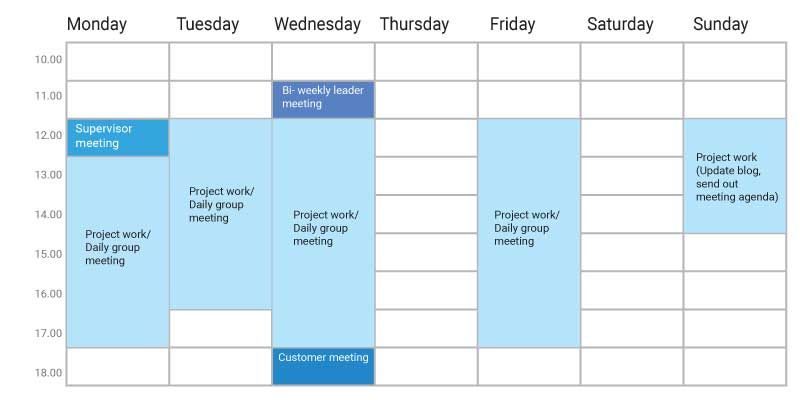
\includegraphics[height=5cm]{figs/WeeklySchedule.jpg}
\caption{The weekly schedule}
\label{fig:weekly-schedule}
\end{figure}

\subsection{Meeting objectives}
In this section the purpose of the different meetings are described. In addition to the meetings shown in figure \ref{fig:weekly-schedule}, the team will have version meetings at the start and end of every version. 

\begin{description}
    \item[Stand-up meetings] \hfill\\ 
     To confirm that there is a progress in the project, and identify problems that occurs, daily stand-up meetings will be held. The stand-up meetings are derived from Scrum, where each team member describe what is done since last stand-up, what will be done before the next stand-up and potential problems they have encountered. \cite{scrum} 
   
    \item[Supervisor meetings] \hfill\\ 
    In the supervisor meetings, where the team and supervisor participates, the objective is to discuss progress of the project. Both of the product and of the process around working as a team. The team will also receive feedback on the work done since last meeting.
    
    \item[Customer meetings] \hfill\\ 
    The main purpose of the customer meetings is for the team to present the progress of the product. The progress from the previous meeting will mainly be presented as videos. The videos are created by recording the application preforming selected tasks, and are distributed on YouTube for the customer to watch.
   
    \item[Version meetings] \hfill\\ 
    Working with fast iterations without much planning, it is important for the team members to feel they can contribute to improve the process. This is the objective of version retrospective meetings. Execution of these meetings are described in section \ref{retrospective-intro}.
    Before starting the development of a new version, the team will have a planning meeting where the goal is to select what is the most important assumption to be tested. The conduction of this phase is described in section \ref{planning-intro} 

\end{description}
 
\section{Quality assurance}
To assure quality in the project some guidelines were set to improve both the communication, and productivity. These include time of response, meeting templates and version control, in addition to standards set for files, 

\subsection{Time of response}
Communication is crucial in a group.\cite{teamwork} To make sure that a team member can expect an answer within a limit of time, a maximum response time is set to 24 hours. This limit applies to internal communication in the team, as well as between the team and the supervisor and the customer representative.

\subsection{Meeting routines}
To make sure that the quality of the meeting minutes held the desired standard, the team designed a set of templates. The meeting templates for the supervisor and customer meetings are shown in appendix \ref{app:templates}, section \ref{app:supervisor-template} and \ref{app:customer-template} respectively.
The team, in collaboration with the customer representative and supervisor respectively, decided routines for the meetings. These are described in the following sections.

\subsubsection{Routines for customer meetings}
  Before meeting with the customer representative, he should be invited to the meeting and a meeting agenda should be ready. The meeting agenda should be updated to contain the present status of the project, and potential questions from the group. 
  After the meeting, he should be able to review the meeting minutes. 
  The customer will be called to meetings by creating a new event in Google Calendar, and inviting the customer. This should be done at least 24 hours before the meeting is held.
  Review of the meeting minutes is done by uploading the minutes to a shared folder in Google Drive after the meetings. %Tom for luft

   		
\subsubsection{Routines for supervisor meetings}
  The supervisor should receive a meeting notice within 24 hours prior to the meeting, which in this project is by Sunday at 12.15. The calling for meeting includes the meeting agenda, the report and the meeting minutes of last supervisor meeting and customer meeting. Google Drive will be used to share these documents. In addition, a link to the weekly blog post is added to the agenda, and is used to describe the current status.

\subsubsection{Routines for internal meetings}
 The stand-up meetings are held each day the team work together. This will assure quality by confirming that all team members do their work. In addition to these meetings, the team will have a retrospective meeting after each version to assure that all team members have the opportunity to share what they think works well and more importantly what they think can be improved.
   		  

\subsection{Version control}
Git and GitHub will be used for version management.\cite{git-hub} A CrowdShelf organization was created on GitHub where all code will be pushed. The organization contains four repositories: the Android application, the iOS application, the backend and the web page. Using GitHub enables all code to  be available to all members of the group, and easy, cloud-based version control. The code base will also be available to the customer, or anyone else who wants to use it.

Across all the repositories there is a general workflow to utilize git and GitHub to the fullest. In each of the repositories there is a master \gls{branch} called \code{master} where all releases will be stored. In other words: The \code{master}-\gls{branch} is the base for the \gls{prodenv}. In addition, there is a development \gls{branch}, called \code{dev}, where the latest bug free code will be pushed. This \gls{branch} is the base for the \gls{devenv}. There's made a new \gls{branch} for each new feature. When a feature is completed and bug free, it can be merged to the developing \gls{branch}. Therefore, the developing \gls{branch} will always contain an up-to-date runnable code.

An important part of version control is the message tied to a commit, the ''git commit message''. All the development teams have been trying to follow a good git commit practice, based on ''the seven rules for a good git commit message''.\cite{git-commit}

\subsection{Code standards}
All the teams will follow some code style guidelines to make the code easier to understand and use. The Android team will try to follow guidelines from an web site on Android developing.\cite{android-standard}. The iOS team will try to conform to the guidelines defined by 'raywenderlich.com'.\cite{ios-standard} As for the backend solution, it is written in JavaScript. JavaScript can be written in many ways, but the team chose Crockfords style guide as the code standard for the project.\cite{crockford}

\subsection{File name standards}
In addition to following the code standards, the sub-teams have some standards for naming the code files. The mobile-teams will name their models according to their respective counterparts defined in backend. All class files will be named in the format of pascal case.\cite{pascal-case} Views should be named by combining what kind of data or functionality it will represent, and with what kind of view it is. This means that the view for logging in will be called \code{LoginView}. The \code{LoginView}'s controller will be called \code{LoginViewController} in iOS, and \code{LoginActivity} in Android. Methods are named using camel case.\cite{pascal-case}

\subsection{Document standards}
Files that are not directly linked to the development of products will be stored in Google Drive.\cite{google-drive} These files include files such as meeting minutes, results from surveys and tests, different photos and figures, contact information and time sheets. This will assure that no information is lost, and gives all stakeholders of the project access to all data generated.

\subsection{Issue and task management}
To keep track of what is being done and the progress during each version, the team will use Atlassian's issue tracking software called JIRA.\cite{jira}. All issues will be organized in a kanban board (figure \ref{fig:kanban-illustration}).\cite[p. 137]{lean-startup} All tasks should be added as issues in the \gls{backlog} as they appear. If an issue is related to the current version, it is placed in the "Selected for Development"-column. When someone starts working on an issue they will move it to the "In progress"-column. When an issue is ready to be tested, it is moved to the "Validation"-column, and finally to the "Done"-column when it is complete. By following these standards, it will be easier for the team leader monitor the progress and identify potential bottlenecks.

\begin{figure}
    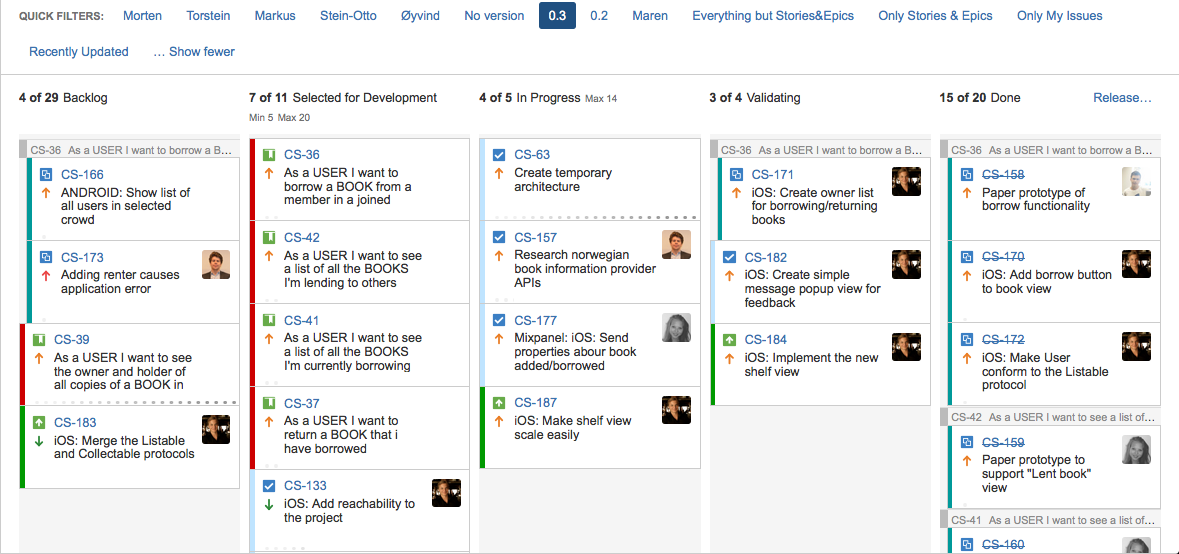
\includegraphics[width=\textwidth,keepaspectratio,origin=c]{figs/kanban-illustration.png}
    \caption{The kanban board used to organize the JIRA issues}
    \label{fig:kanban-illustration}
\end{figure}

\subsection{Design standards}
When developing a system for a specific platform, it is desired to follow design guidelines which helps making the \gls{UI} familiar to the user who is already familiar with the \gls{OS}. When designing an \gls{API} the focus on usability is desirable , as you want it to be easy to understand, and also that the developers using it can find it easy to use, based on \gls{API}s they've used before. 

\subsubsection{Mobile applications}
In general, the team wants to adhere to the platform-specific guidelines as close as possible. This comes at the expense of the applications looking identical across the two platforms iOS and Android, but the differences should not make it hard for users familiar with one platform to switch to the other.  

The iOS team will be following Apple's Human Interface Guidelines to ensure that the application design conforms to the platforms general design.\cite{human-interface-guidelines} The team will also get inspiration from other applications' solutions to similar problems as they appear.

The Android team will be following material design guidelines from the homepage of Android developing.\cite{android-design} In addition, inspiration can be gathered from popular Android application to choose a design that the users is comfortable with.

\subsubsection{\gls{API} standards}
To assure quality in the \gls{API}, the backend team decided, together with the customer representative, to develop an \gls{API} that conforms to the \gls{REST}-standard. \gls{REST} is a software architectural style developed by Roy Thomas Fielding.\cite[chap. 5]{fielding2000} With REST one designs the requests to be stateless, that is each request is separate of any other request. Each component, the client and the server, keeps track of its own state. In practice a RESTful API is built on the \gls{HTTP}, and the \gls{HTTP}-methods that already exist. From there one designs \gls{URL} for the different resources, and operations on them.\cite{rest-web-services} The White House has written a standard for REST over \gls{HTTP}, which describes what the URLs should look like.\cite{whitehouse-api-standard} The team also looked at RESTful APIs that work over HTTP, which big companies has made, such as GitHub and Twitter.\cite{github-api}\cite{twitter-api}

The main point is to base operations around the entities that the components operate on. In the case of CrowdShelf, that means users, books and crowds. Based on this, the root URL's would be \url{/users}, \url{/books} and \url{/crowds}. Combined with \gls{HTTP}-methods, this makes out some basic \gls{CRUD}-operations: A \code{POST}-request to an entity, is for making a new one.\cite{http-method-spec} If you add an \gls{ID}-number after the entity, you can do either a \code{GET} to get the data, or \code{PUT} to update the data. \code{DELETE} will delete the entry. Using the same HTTP-methods and adding operation after the \gls{ID}-number, will do operations on that entity. For example to add member to a crowd you can \code{PUT} a user id to the URL \url{/crowds/crowdID/member/userID}. Do a \code{DELETE} request to the same URL to remove the member from the crowd.


\section{Tools}
This section contains a short description of the tools used for project organization. A tabular description of the tools is shown in table \ref{org-tools}.

    \subsection{Google Drive}
    Google Drive is a file storage and synchronization service created by Google \cite{google-drive}. 
    Google Drive is being used to share movies, sketches and other files that all the people involved in the project should have access to.
    \subsection{Google Docs}
    Google Docs is a part of Google's web based office suite.\cite{google-docs} In this project Google Docs is used to write the meeting minutes and the hour list because it is an easy way to share documents and keep them synchronized.
    \subsection{JIRA}
    JIRA is an issue tracking system created by Atlassian.\cite{jira} With JIRA's version and issue functionality it is easy to see who is working on what task, or how a version is coming along. This project will use JIRA's kanban board to keep track of the work that is being done.\cite[p. 137]{lean-startup} It also includes smart filters that makes it easy to keep track of what individuals are working on, and in what version tasks are created. In each version the team will generate user stories to describe the version's functionality. The team will then add all the tasks that must be done in order for the selected user stories to function in the application.
    
    \subsection{Share\LaTeX}
    \LaTeX is document markup language that let's us define the structure and content of the report, without having to worry about how it looks, which the \LaTeX-compiler takes care of for us.\cite{latex} ShareLaTeX is an online and interactive \LaTeX-editor.\cite{share-latex}
    In this project Share\LaTeX is used for the report writing. It was chosen because it allows real time collaboration on the \LaTeX-code.
    \subsection{Git/GitHub}
    Git is an open source version control system.\cite{git} Git is used in this project in combination with GitHub which is a web based Git repository service.\cite{git-hub} Git allows the team to easily work together on the same system.
    \subsection{Slack}
    \label{about-slack}
    Slack is a messaging application for teams.\cite{slack} Everyone in the group registered in the CrowdShelf team, and the customer contact was invited, who in turn invited colleagues from Netlight to participate. Slack allows the team, to have different channels for different purposes, such as design, report writing and one for each of the development teams. This is used to coordinate and discuss topics between meetings. It also allows direct messaging between members, making all communication centralized. In addition, it integrates with both GitHub and JIRA so that updates in these tools are also added as a message in the Slack application.

\begin{table}[]
\centering
\begin{tabular}{|L{2cm}|L{2cm}|L{4cm}|L{3cm}|L{4cm}|}
\hline
\textbf{Purpose of Use} & \textbf{Tool} & \textbf{Description} & \textbf{Source} & \textbf{Notes} \\ \hline
To share files in the project. & 
Google Drive & Google Drive is a file storage and synchronization service created by Google & 
www.google.com/ intl/en/drive & 
This project shares a folder in Google Drive where all the files created are stored. \\
\hline
To share documents and keep them synchronizes. & 
Google Docs & 
Google Docs is a web based office suit that includes word processor, spreadsheet and presentation programs. & 
www.google.com/ intl/en/docs/about/ & 
The main use of Google Docs are for the meeting agendas and to create hour lists and other spreadsheets. \\
\hline
To keep track of the tasks and user stories of the software project. & 
JIRA & 
JIRA is an issue tracking system created by Atlassian & www.atlassian.com/ software/jira & 
In JIRA the main application is a Kanban board to keep track of the user story backlog and the tasks created for each version. \\ \hline

To write the report. & 
Share\LaTeX & Share\LaTeX is an online and interactive \LaTeX-editor & 
latex-project.org/ intro.html www.sharelatex.com/ & Share\LaTeX is only used for the report because of the some what demanding structure of \LaTeX. \\\hline

To obtain version control. & 
Git \& GitHub & 
Git is an open source version control system. GitHub is a web based Git repository hosting service. & 
git-scm.com/ github.com/ & 
The project has a public repository located at https://github.com/ CrowdShelf \\\hline
To communicate & 
Slack & 
Slack is a team collaboration tool that includes messaging and integration with JIRA, GitHub and Google Docs among others. & slack.com & 
CrowdShelf has a slack-team where the development team and resouces from Netlight including the customer have access.\\ \hline
\end{tabular}
\caption{Table of project organization tools}
\label{org-tools}
\end{table}  
 

\begin{sidewaystable}[]
\centering
\begin{tabular}{|L{3cm}|C{1cm}|C{1cm}|C{.75cm}|L{6cm}|L{9cm}|}
\hline
\textbf{Description} & \textbf{\begin{tabular}[c]{@{}c@{}}P.\\ (1-10)\end{tabular}} & \textbf{\begin{tabular}[c]{@{}c@{}}C.\\ (1-10)\end{tabular}} & \textbf{\begin{tabular}[c]{@{}c@{}}Risk \\ value\end{tabular}} & \textbf{Prevention} & \textbf{Solution} \\ \hline
Task not completed & 4 & 6 & 24 & Ensure estimates are adequate, and allocate sufficient resources for tasks & Work extra hours to complete the task \\ \hline
Absence (+4 days) & 4 & 5 & 20 & If a group member is going away it must be notified in advance & If we know that a group member is leaving we can assign tasks that can be done \\ \hline
Can not solve a problem & 5 & 4 & 20 & Good internal communication in the team will prevent most problems & Consult advisors, customer or course staff \\ \hline
Loss of data & 3 & 6 & 18 & Use version control and online backups for all documents and resources & Restore backup.  \\ \hline
Computer malfunction & 2 & 8 & 16 & Keep software updated. & Try to find a new computer for the team member \\ \hline
No feedback from users & 2 & 8 & 16 & Try to reach users through multiple channels like the customer, Reddit, Facebook and more & Contact family and friends \\ \hline
Conference room unavailable & 5 & 3 & 15 & Book rooms in advance & Find a quiet spot and conduct the meeting on a laptop \\ \hline
Missing competence & 5 & 3 & 15 & Map team members competence and preferred technologies & Find alternative solutions if possible. If not, allocate resources for team member to learn the new technology \\ \hline
Illness & 7 & 2 & 14 & Try to prevent taking unnecessary health risks. & Divide the team members task among the team members \\ \hline
Latecomers & 7 & 2 & 14 & Make sure all team members know when meetings will take place through calendars and messages & The latecomer will have to work additional hours to make up for lost time. The team member should also communicate its status by other means if possible \\ \hline
Miscommunication & 2 & 6 & 12 & Clearly define all tasks and who is responsible for their execution & Find out what has been done and reorganize. \\ \hline
Apple disapproves the app & 2 & 6 & 12 & Make sure not to use private APIs and follow Apples guide lines & Update what is preventing the app from being approved and submit for review \\ \hline
Loss of team member & 1 & 9 & 9 & Make sure all team members feel included and are in good health & Distribute the late team members tasks among the remaining team members. Revise the project plan and remove the least important tasks if necessary \\ \hline
Force majeure & 1 & 7 & 7 & Good communication & Work individually and arrange meetings when possible \\ \hline
Unreachable version control server & 1 & 5 & 5 & Store versions locally to be able to keep working. & Keep editing local revisions and push when the service is back online. Communicate to avoid redundancy and conflicts \\ \hline
\end{tabular}
\caption{Risk assessment}
\label{table:risk-assessment}
\end{sidewaystable}

\section{Risk management}
The team chose to keep track of the risk assessment by making a risk matrix with risk values, prevention methods and solutions if a risk would occur. Table \ref{table:risk-assessment} contains a description of each risk, a scale of one to ten indicating how probable this risk could occur, a scale of one to ten indicating how severe the consequences would be if this risk occurred. A risk value is calculated by multiplying the probability value by the consequence value. This value is also shown in the table together with methods to prevent the risk from occurring, and possible solutions if a risk occurs.


